\documentclass[convert={outfile=mlp_model.svg}]{standalone}

% Now include my standard packages, which also includes:
\usepackage{standalone}
\usepackage{tikz}
\usetikzlibrary{matrix,chains,positioning,decorations.pathreplacing,arrows}

\begin{document}
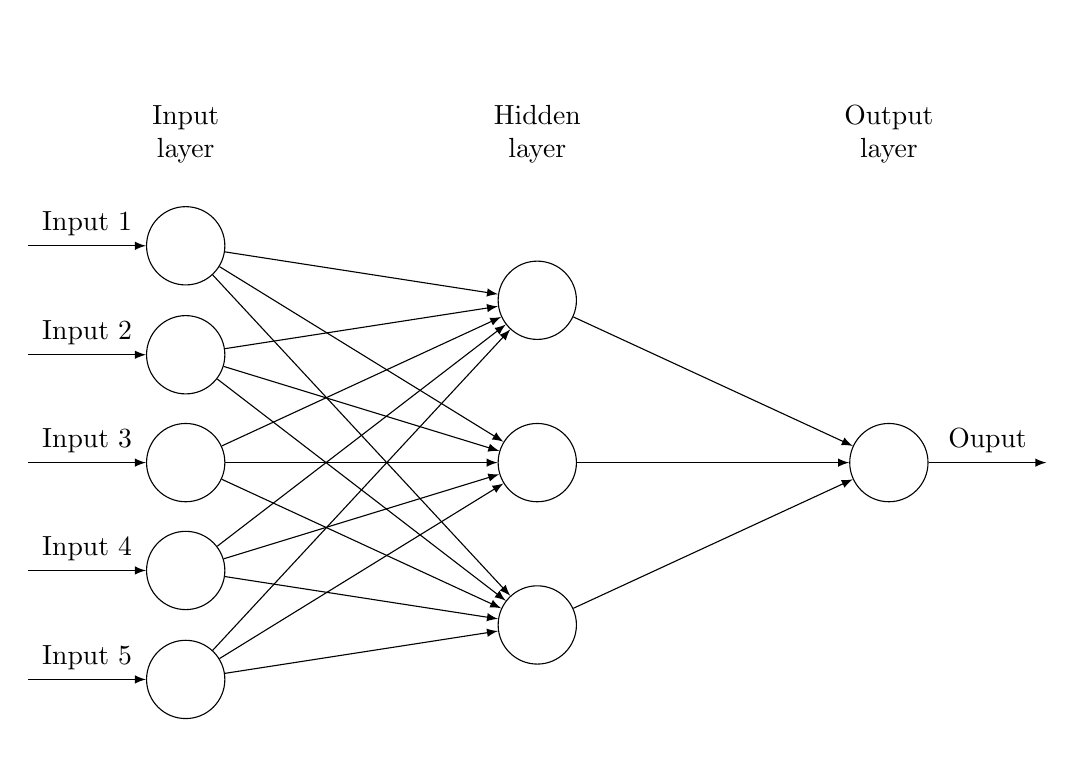
\begin{tikzpicture}[
    plain/.style={
        draw=none,
        fill=none,
        },
    net/.style={
        matrix of nodes,
        nodes={
        draw,
        circle,
        inner sep=10pt
        },
        nodes in empty cells,
        column sep=2cm,
        row sep=-9pt
        },
    >=latex
    ]
    \matrix[net] (mat)
    {
    |[plain]| \parbox{1.3cm}{\centering Input\\layer} & |[plain]| \parbox{1.3cm}{\centering Hidden\\layer} & |[plain]| \parbox{1.3cm}{\centering Output\\layer} \\
    & |[plain]| \\
    |[plain]| & \\
    & |[plain]| \\
        |[plain]| & |[plain]| \\
    & & \\
        |[plain]| & |[plain]| \\
    & |[plain]| \\
        |[plain]| & \\
    & |[plain]| \\    };
    \foreach \ai [count=\mi ]in {2,4,...,10}
        \draw[<-] (mat-\ai-1) -- node[above] {Input \mi} +(-2cm,0);
    \foreach \ai in {2,4,...,10}
    {\foreach \aii in {3,6,9}
        \draw[->] (mat-\ai-1) -- (mat-\aii-2);
    }
    \foreach \ai in {3,6,9}
        \draw[->] (mat-\ai-2) -- (mat-6-3);
    \draw[->] (mat-6-3) -- node[above] {Ouput} +(2cm,0);
    \end{tikzpicture}
\end{document}